\section{Interfejs użytkownika (Zofia Sosińska)}\label{chap:ui}
Projekt interfejsu użytkownika przewiduje tryb podstawowy z zawsze widocznymi elementami oraz dynamicznie pojawiające się okna, wywoływane za pomocą konkretnych klawiszy. 
 Zadaniem każdej składowej będzie odzwierciedlenie pewnego fragmentu aktualnego stanu wiedzy granej postaci z naciskiem na najpotrzebniejsze w danej chwili informacje. Przewidziane są:
 \begin{itemize}
    \item menu stawiania budynków; 
    \item menu wydawania komend;
    \item menu zapisu;
    \item informacja o możliwej interakcji;
    \item dziennik z zadaniami;
    \item ekran końca gry.
\end{itemize}
	
\subsection{Interfejs podstawowy}
Interfejs podstawowy przewiduje funkcje, takie jak pokazanie:
\begin{itemize}
    \item aktualnego czasu w grze, aby stworzyć iluzję upływającego czasu w świecie gry; 
    \item surowców i funduszy, aby użytkownik nie był obarczony kalkulacjami przy każdym zakupie lub przypływie zasobów;
    \item kompasu, aby ułatwić nawigację;
    \item stan zdrowia gracza, aby zasygnalizować mu, czy przypadkiem nie rozsądniejsze będzie wycofanie się z potyczki;
    \item etap, na którym są przypisane graczowi zadania, aby przypomnieć mu, że na takowe się zgodził.
\end{itemize}
Inspiracją dla górnego paska z informacjami jest ten użyty w grze Warcraft 3 (por. \ref{c:elem_ui}). Prostota i surowość stylu będą współgrać z klimatem gry.

W naszej grze skupimy się jednak na tym, aby interfejs użytkownika zabierał jak najmniej miejsca. Dlatego też projekt zakłada, że poszczególne obiekty nie będą ze sobą połączone, a jedynie “dryfować” w przestrzeni.
Jako ważny element tej części UI zawarty zostanie kompas, wzorowany na tym z gry The Elder Scrolls V: Skyrim (por. \ref{chap:skrm}).
\begin{figure}[htbp]
    \centering
    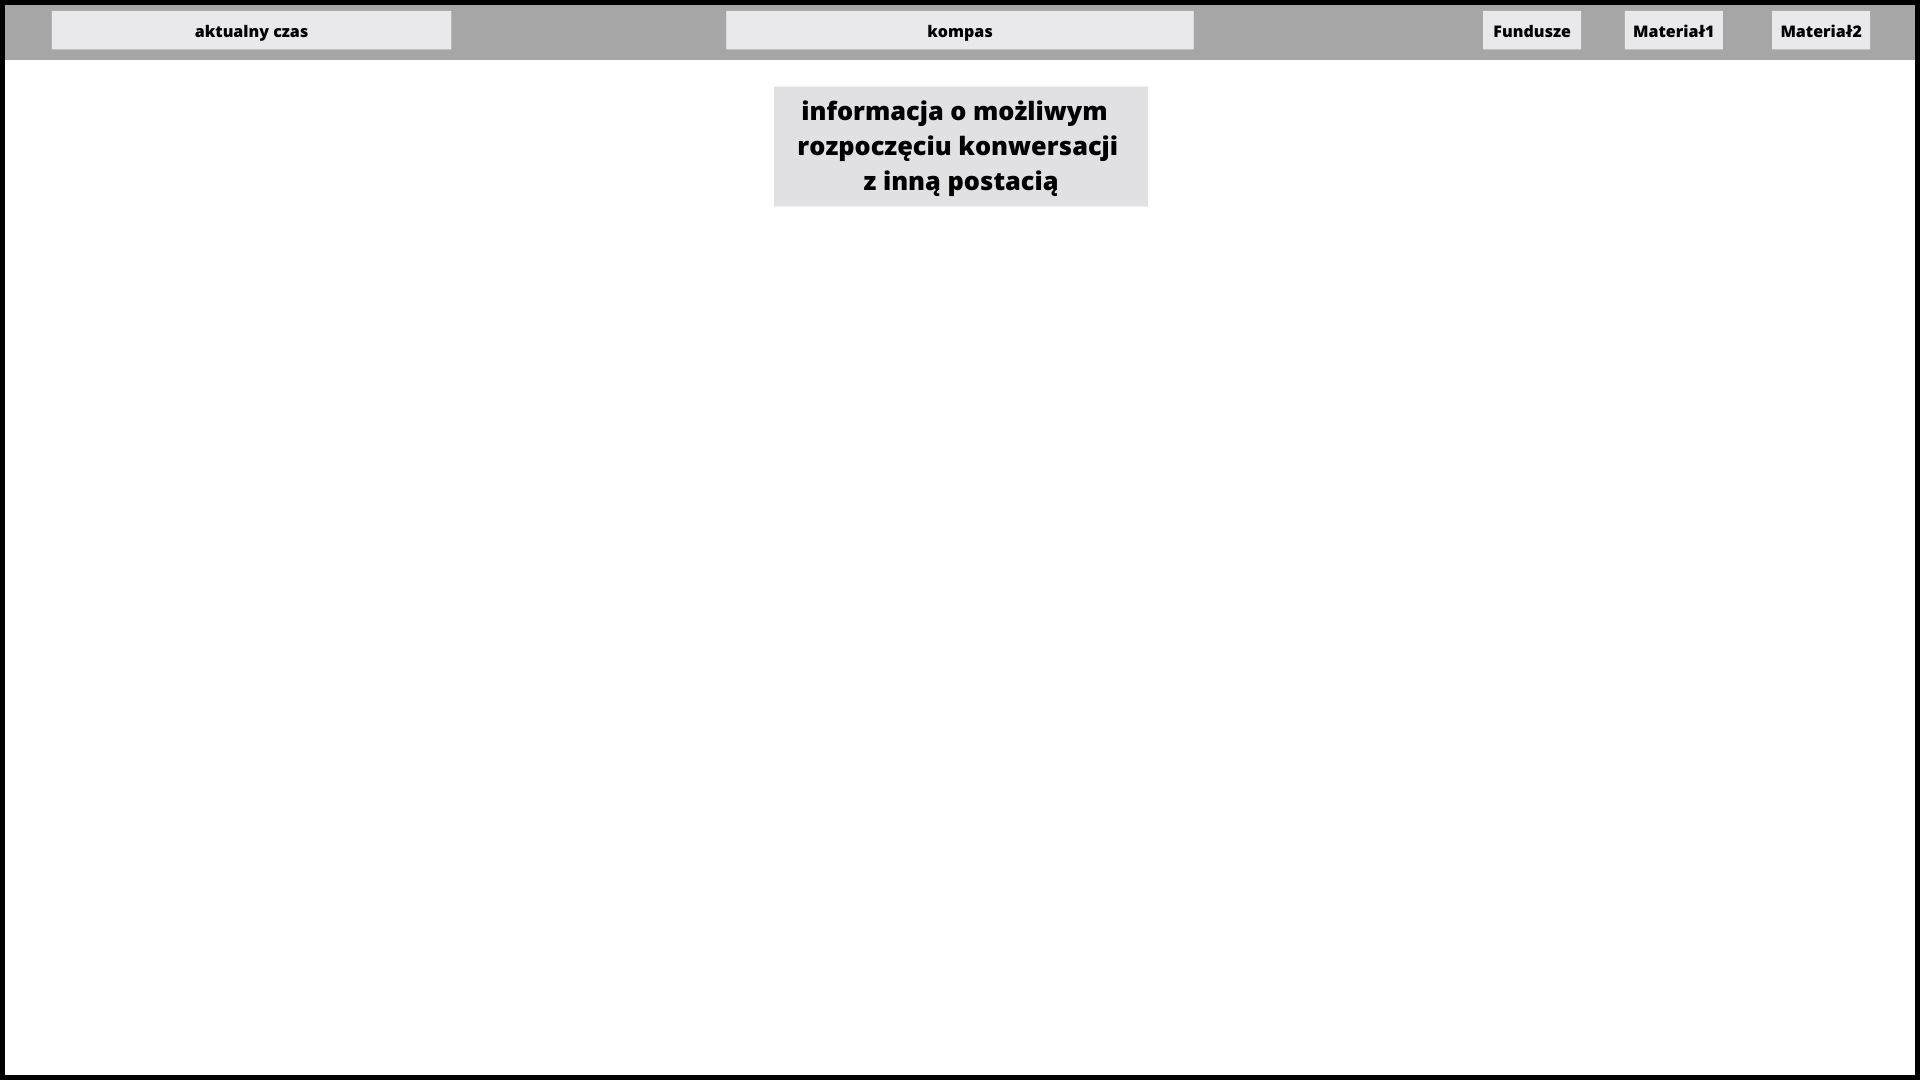
\includegraphics[width=0.9\textwidth]{images/ui/ui_proj_ogolne.jpg}
    \caption{Projekt interfejsu podstawowego UI.
    }\label{fig:ui_main}
\end{figure}
 
\subsection{Menu stawiania budynków}
Menu stawiania budynków będzie obrazować wiedzę i spostrzeżenia głównej postaci przy budowaniu nowej budowli. Docelowym miejscem ukazania się informacji będzie 
dół ekranu, aby interfejs nie zasłaniał użytkownikowi zbyt dużo przestrzeni. Graczowi ukaże się lista dostępnych budynków oraz odpowiednie komunikaty w wypadku, gdy 
nie można będzie dokonać zakupu, czy postawienia. Inspiracją do przedstawienia tych informacji zostanie rozwiązanie gry Orcs must die! (por. \ref{c:elem_ui}).
\begin{figure}[htbp]
    \centering
    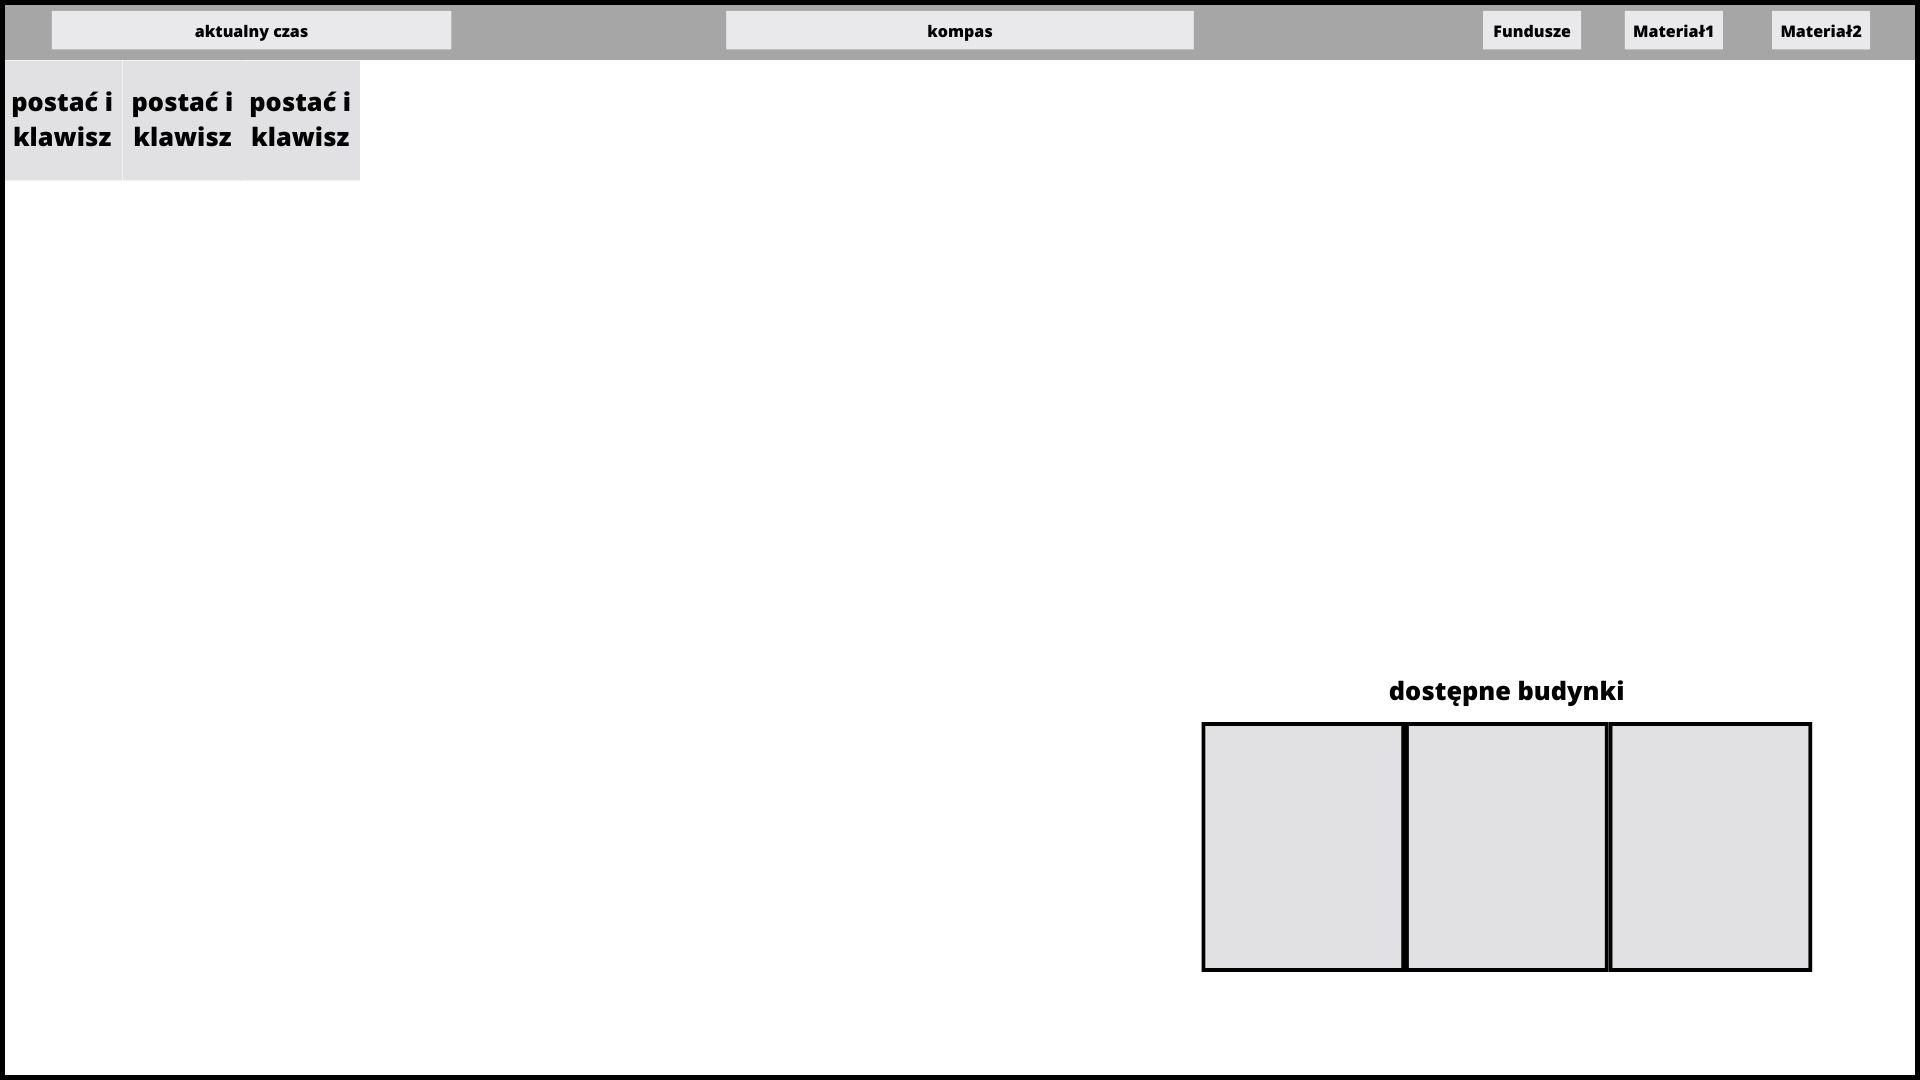
\includegraphics[width=0.9\textwidth]{images/ui/ui_proj_budowanie.jpg}
    \caption{Projekt menu stawiania budynków.
    }\label{fig:ui_bud}
\end{figure}
\FloatBarrier

\subsection{Menu wydawania komend}
Po zdobyciu towarzyszy walki, kluczowe będzie udostępnienie mechaniki sterowania nimi. Zrealizowane to zostanie za pomocą menu wydawania komend.
Projekt przewiduje wyświetlenie listy dostępnych komend i klawiszy, po których naciśnięciu, konkretna opcja zostanie wybrana. 
Źródłem pomysłu jest interfejs zaprojektowany w grze Mount\&Blade (por. \ref{chap:mb}).

\begin{figure}[htbp]
    \centering
    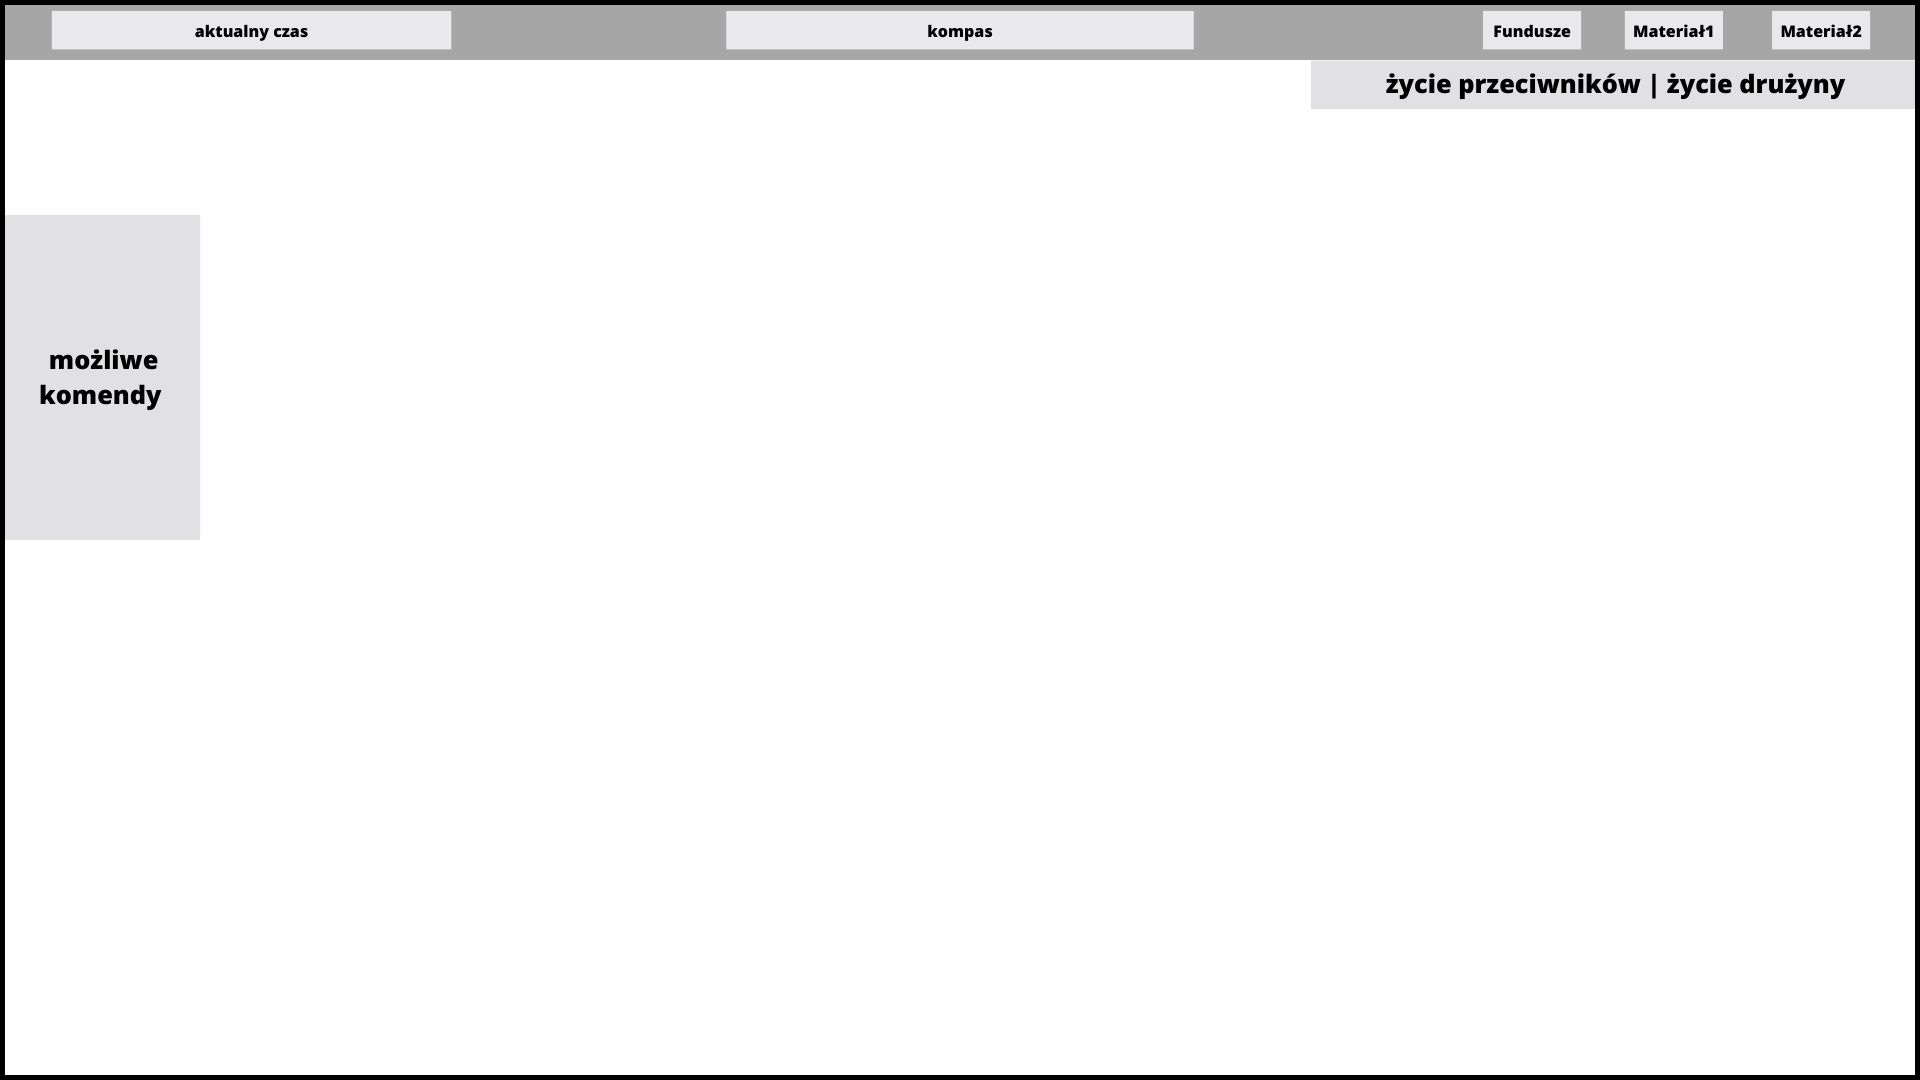
\includegraphics[width=0.9\textwidth]{images/ui/ui_proj_walka.jpg}
    \caption{Projekt menu wydawania komend.}\label{fig:cmd_menu}
\end{figure}
\FloatBarrier

\subsection{Menu zapisu}
Aby umożliwić zapis gry przygotowane zostanie specjalne dla tego zadania menu, wyświetlane na środku ekranu. Najważniejszą informacją 
umiejscowioną na nim będzie nazwa pliku, aby gracz mógł później go odnaleźć.
\begin{figure}[htbp]
    \centering
    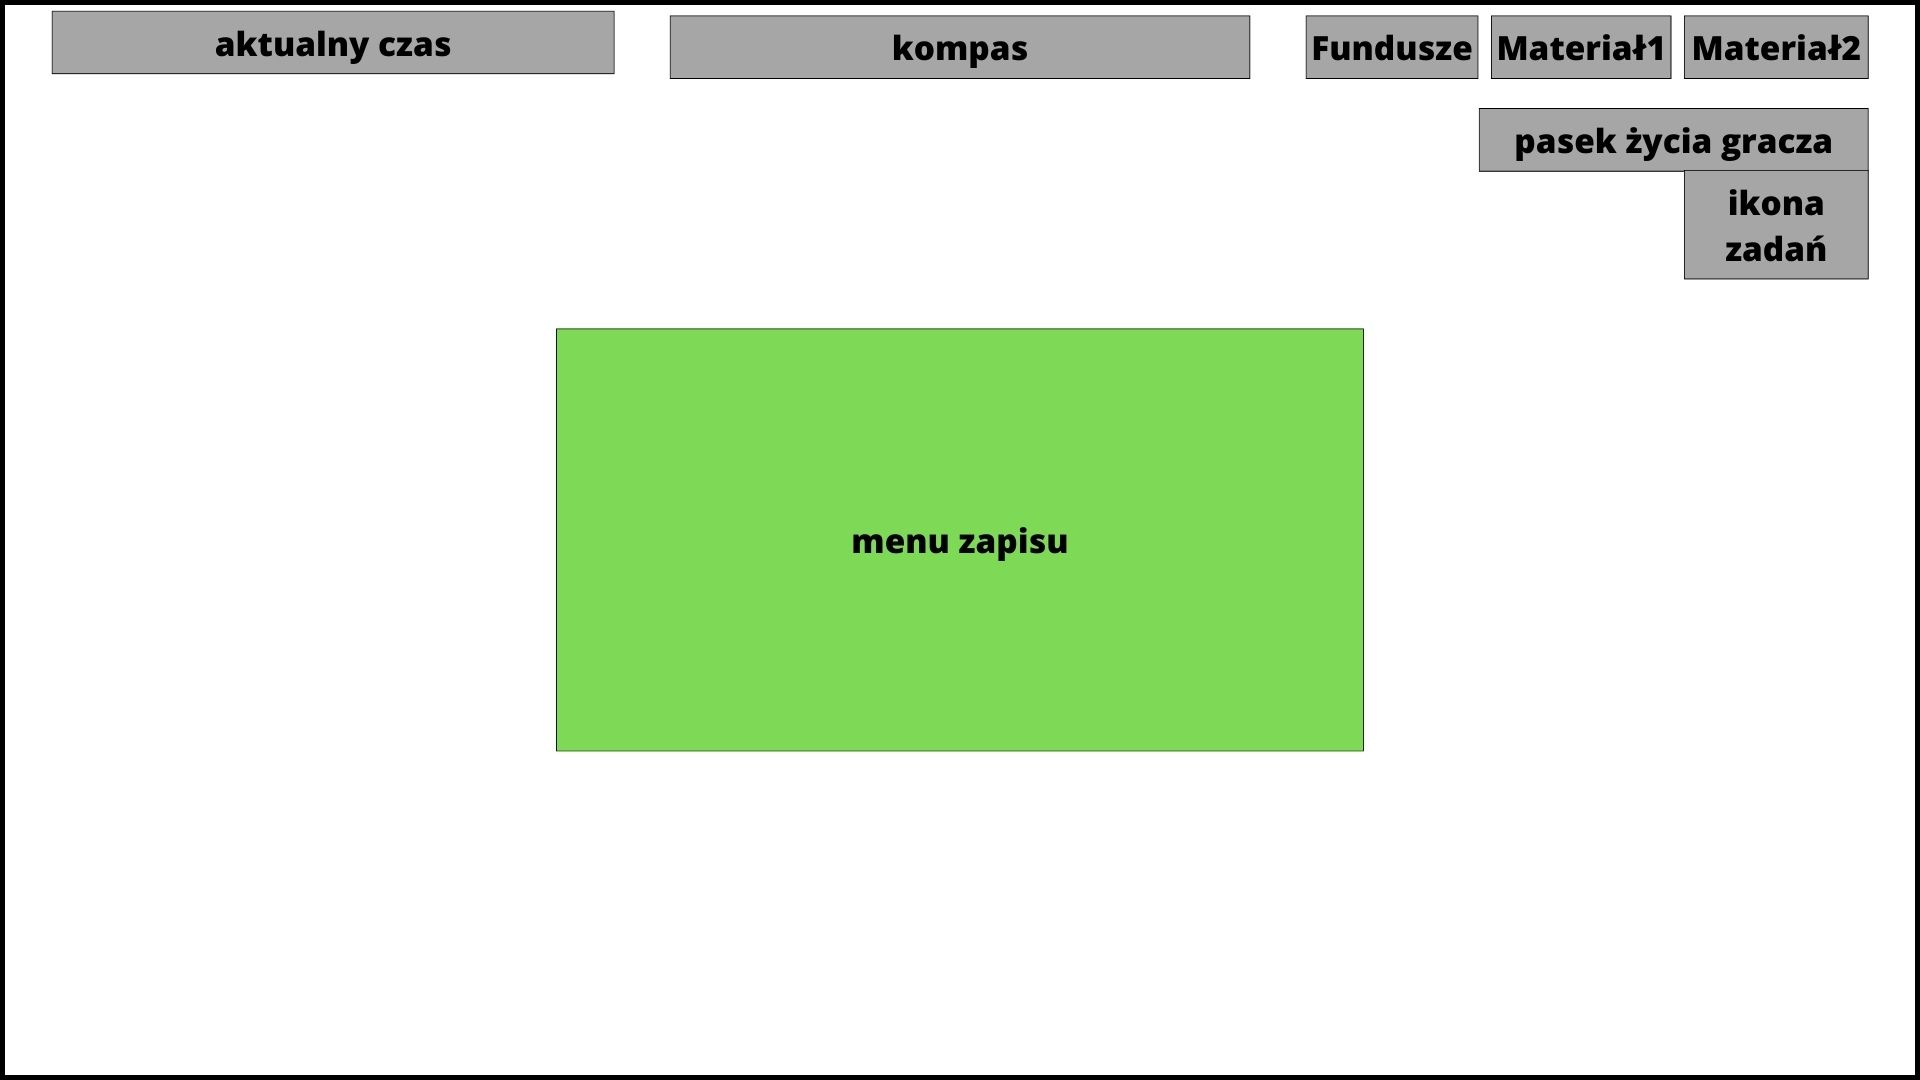
\includegraphics[width=0.9\textwidth]{images/ui/ui_proj_zapis.jpg}
    \caption{Projekt menu zapisu.}\label{fig:men_zap}
\end{figure}
\FloatBarrier

\subsection{Informacja o możliwej interakcji}
W programie przewidziane są postacie i przedmioty interaktywne. Aby zasygnalizowć mu zaistniałą możliwość podjęcia pewnej akcji, 
gra powinna mu wyświetlić stosowny komunikat. Wybranie wysoce widocznego miejsca będzie istotne, ponieważ grafika zniknie,
jak tylko interakcja przestanie być możliwa. Tudzież kluczowe będzie wybranie takiej lokalizacji, aby komunikat zwrócił uwagę gracza nawet, 
jeśli wyświetlony będzie tylko przez krótką chwilę. Za najwłaściwsze umiejscowienie wybrano środek górnej części ekranu, zaraz
pod bazowym interfejsem.
    \begin{figure}[htbp]
    \centering
    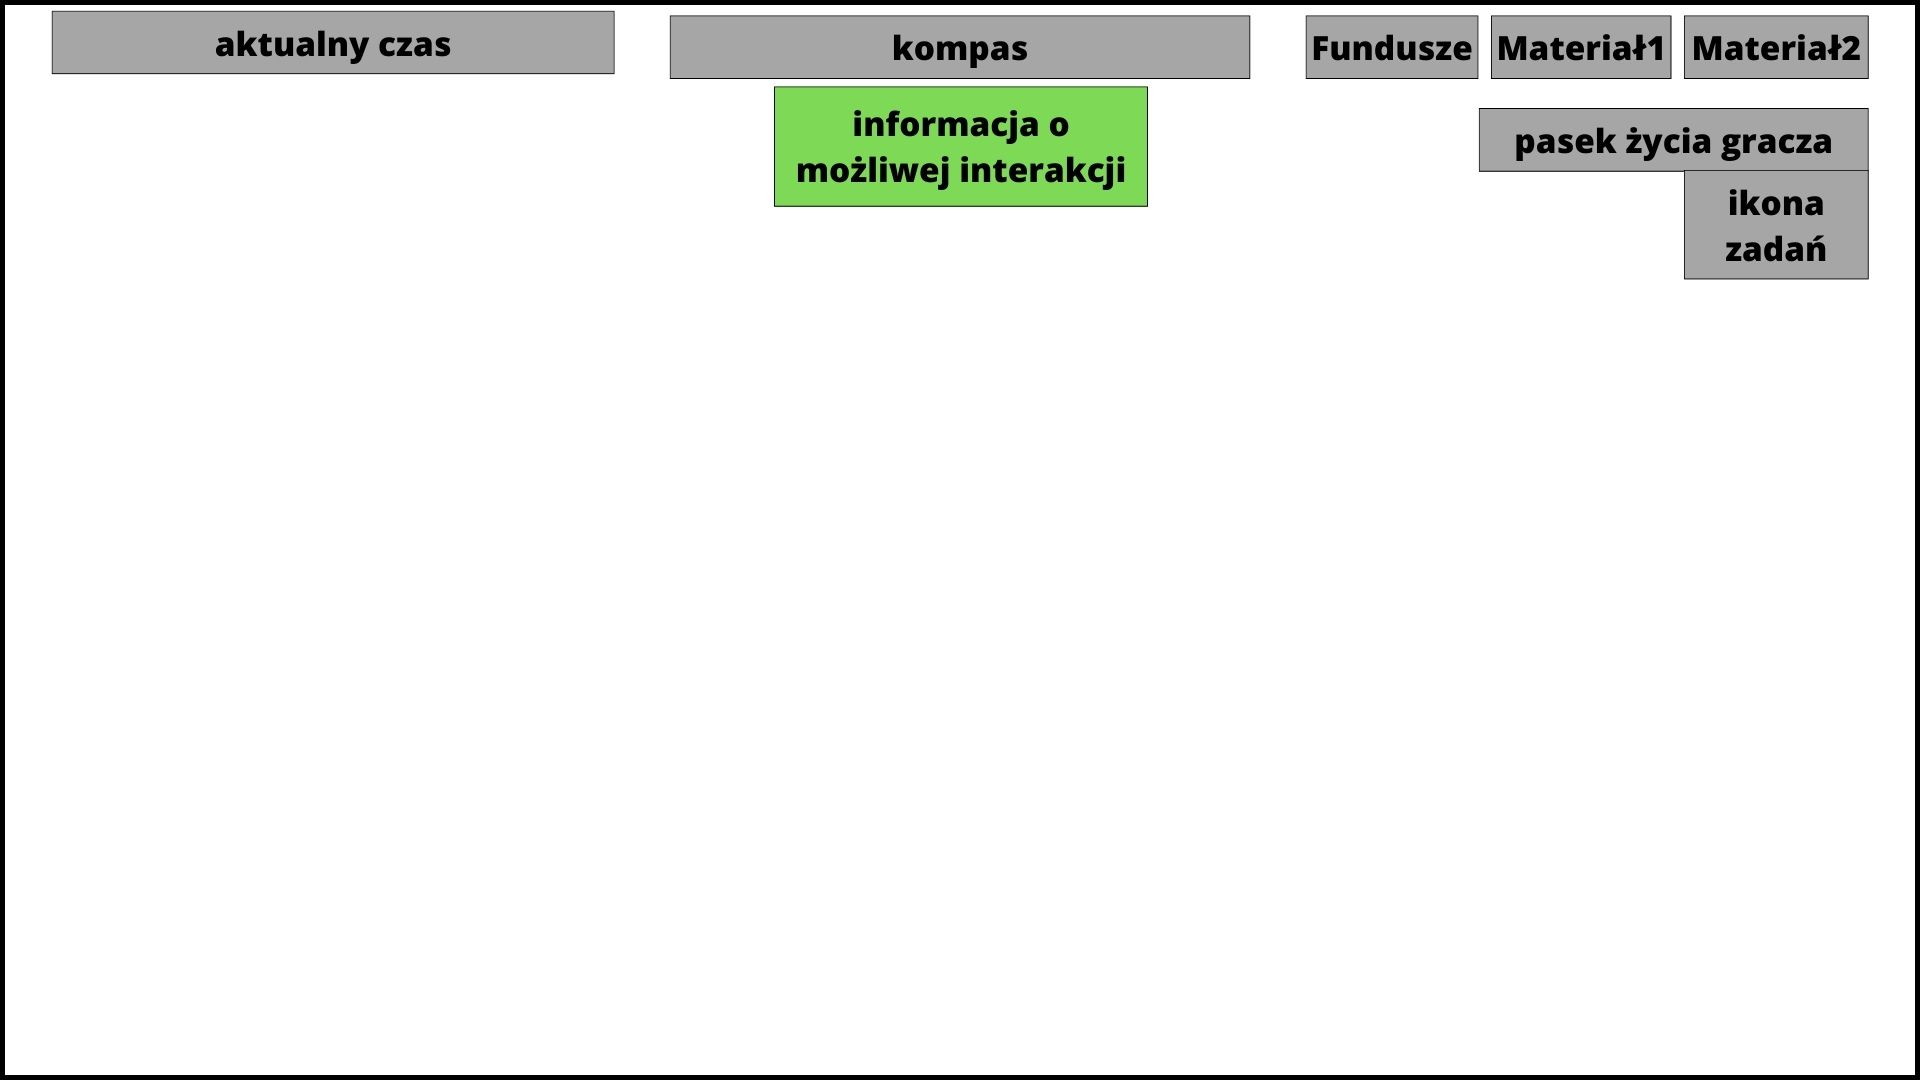
\includegraphics[width=0.9\textwidth]{images/ui/ui_prooj_interakcja.jpg}
    \caption{Projekt grafiki informującej o możliwym rozpoczęciu rozmowy.}\label{fig:rozmow}
\end{figure}
\FloatBarrier

\subsection{Dziennik z zadaniami}
Projektanci systemu zakładają, że niektóre postacie interaktywne będą mogły zlecić graczowi zadanie. Jeśli użytkownik przyjmie wiele zleceń,
to zapamiętanie wszystkich szczegółów może stać się kłopotliwe. Dlatego projekt systemu przewiduje udostępnienie mechaniki dziennika, w którym 
pojawią się informacje o rozpoczętych zadaniach. Na przygotowanej grafice każde z nich będzie miało własne okno ze streszczeniem. Użytkownik 
będzie mógł je przeglądać posługując się suwakiem.
\begin{figure}[htbp]
    \centering
    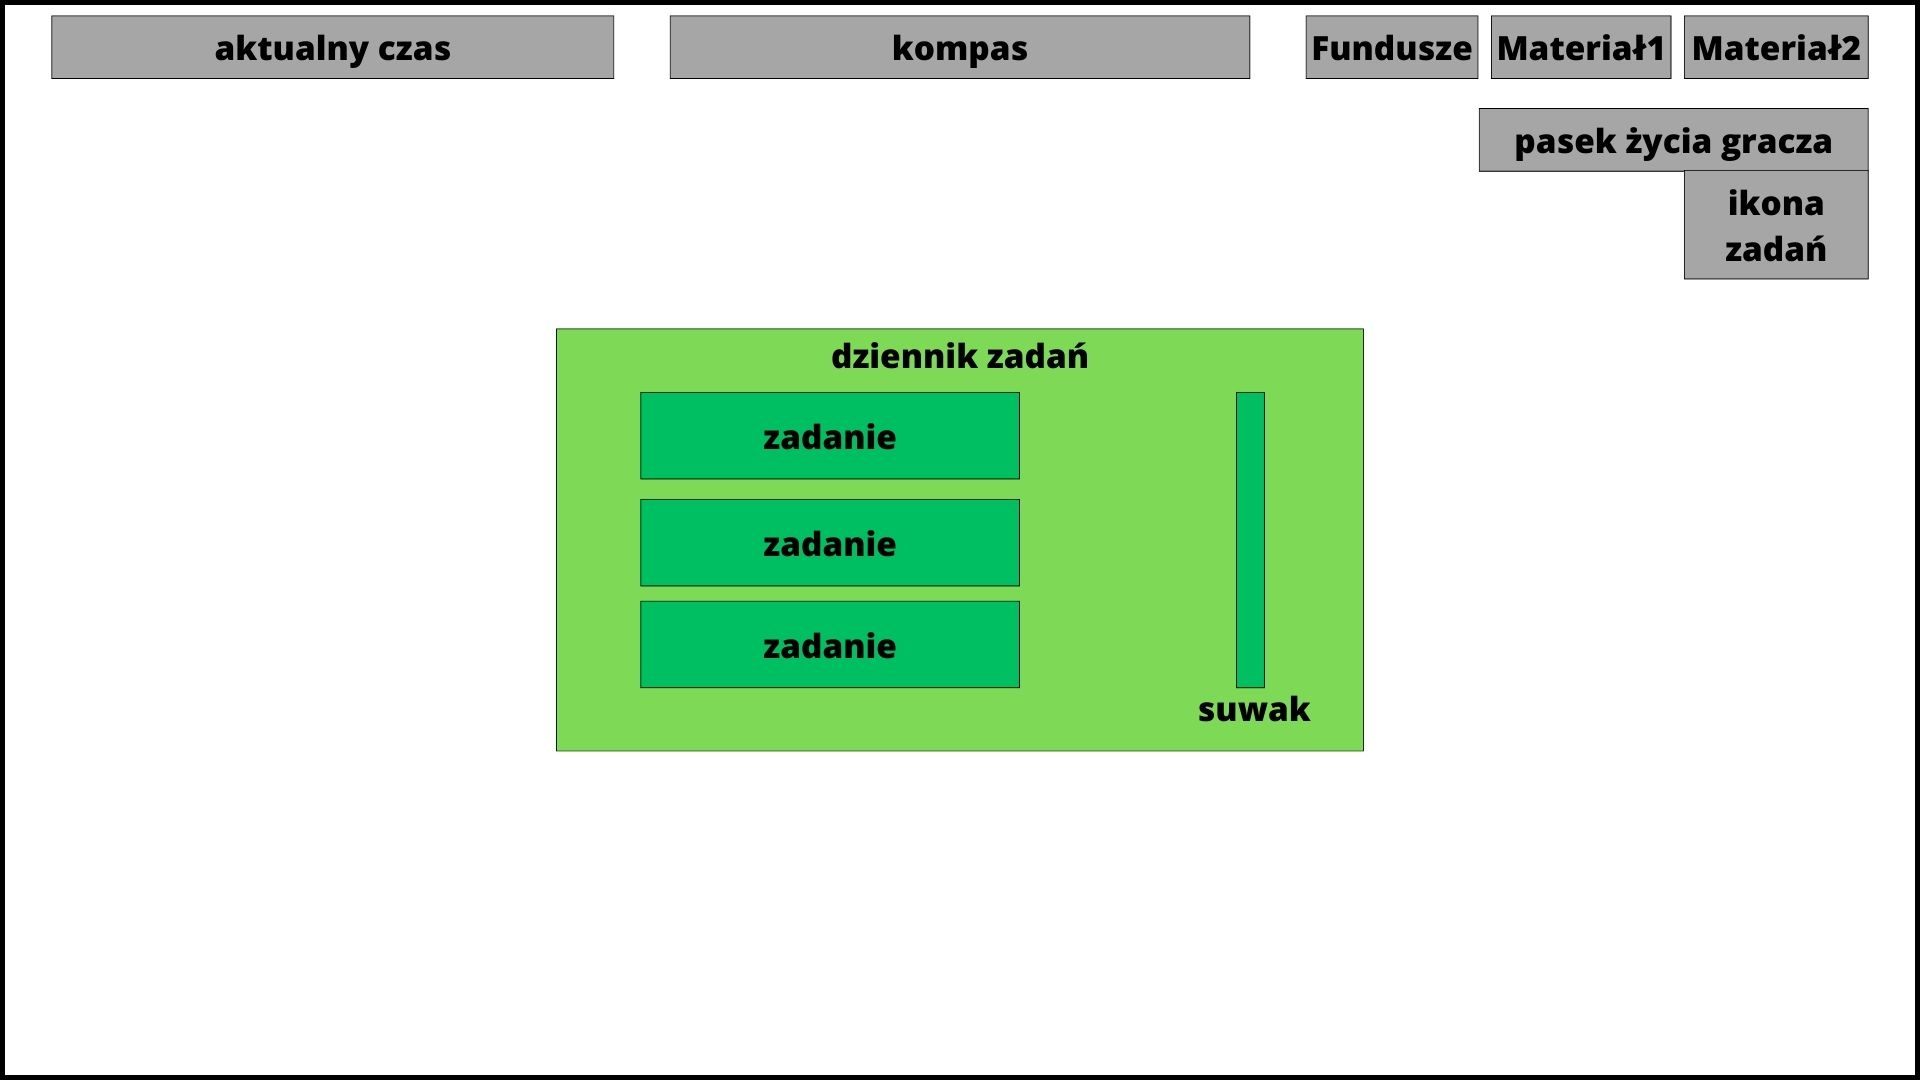
\includegraphics[width=0.9\textwidth]{images/ui/ui_proj_dziennik_zadan.jpg}
    \caption{Projekt dziennika z aktualnie zaczętym i nieukończonym zadaniem.}\label{fig:end_sc}
\end{figure}
\FloatBarrier

\subsection{Ekran końca gry}
Gracz, po wykonaniu pewnych kroków, może doprowadzić grę do stanu końcowego. W takim wypadku przewidziane jest wyraźne tego zasygnalizowanie przez program.
Przewiduje się zaprojektowanie specjalnego ekranu końca gry. W tym celu użytkownikowi zostanie wyświetlona klarowna informacja o aktualnym stanie rzeczy oraz instrukcja,
co zrobić dalej. Dodatkowo, aby wzmocnić przekaz, cały ekran zostanie przyciemniony.
\begin{figure}[htbp]
    \centering
    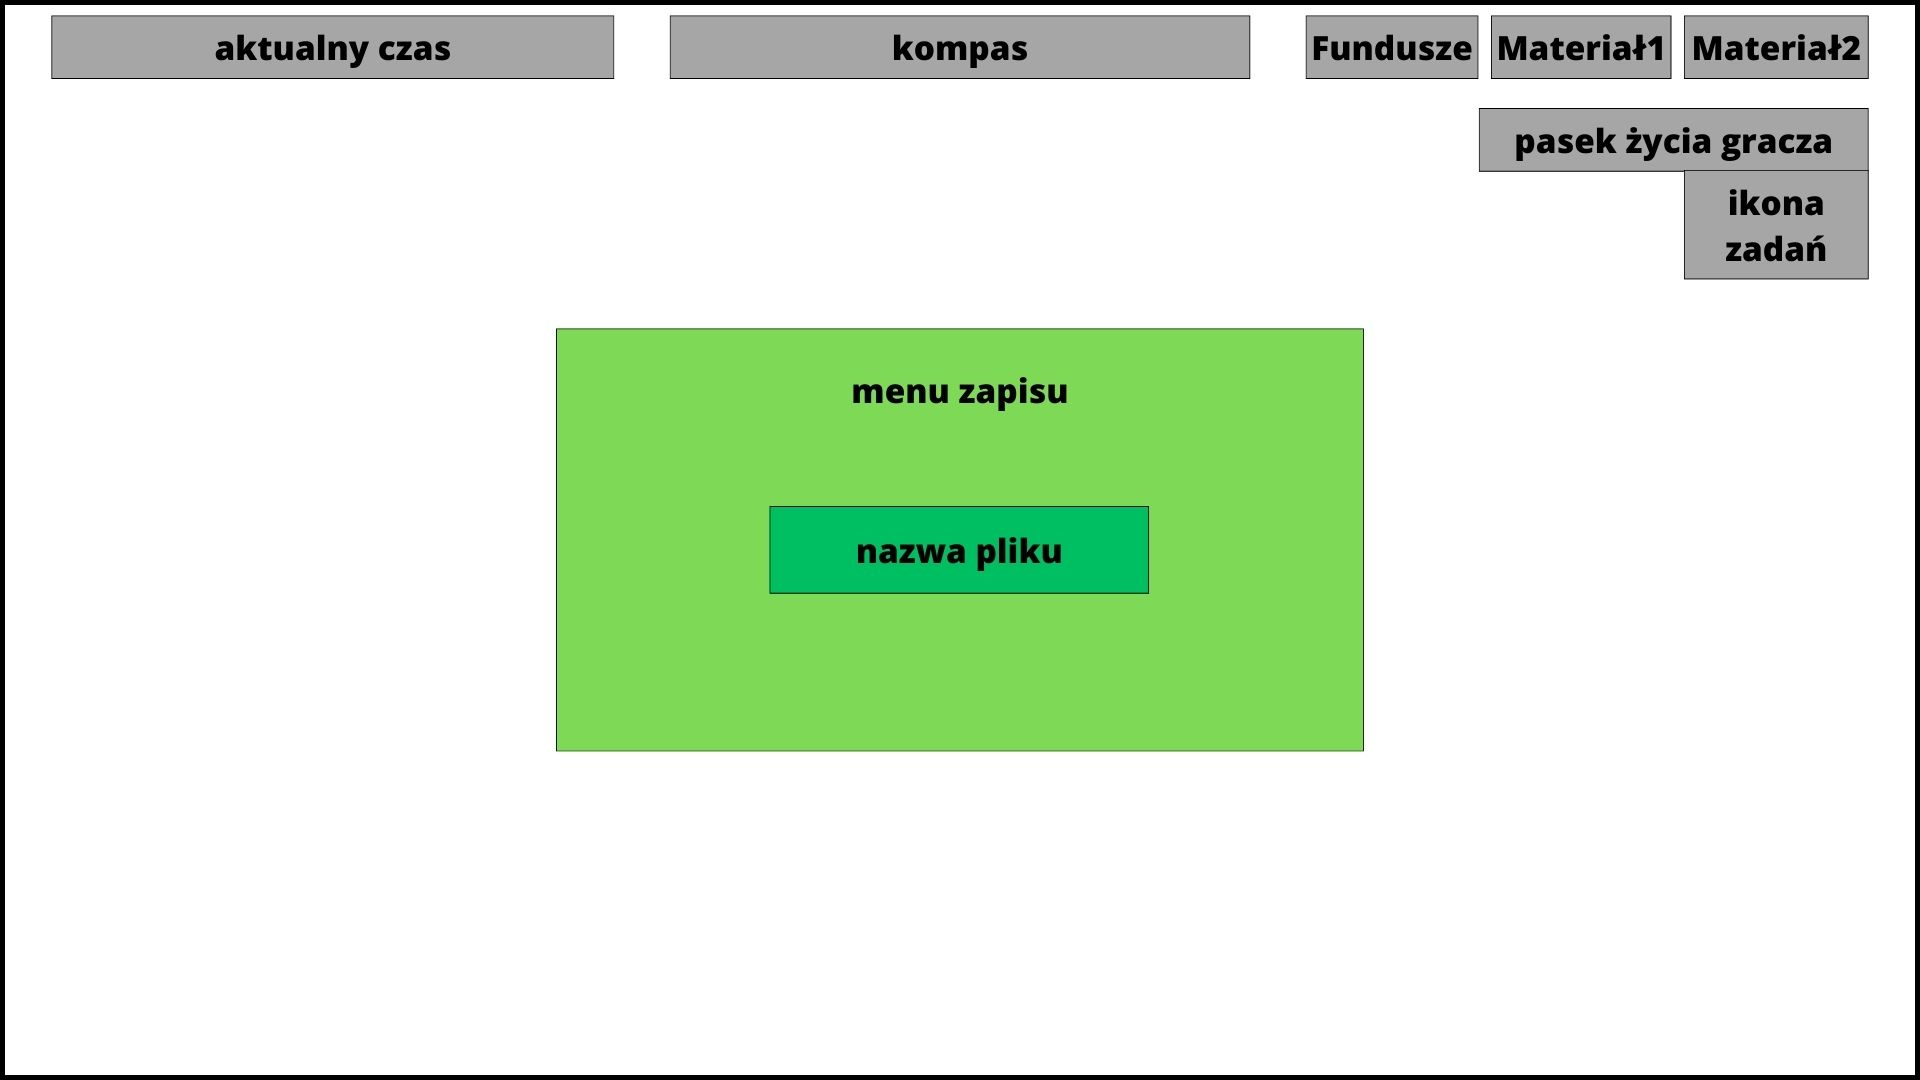
\includegraphics[width=0.9\textwidth]{images/ui/ui_prooj_koniec_gry.jpg}
    \caption{Projekt ekranu końca gry.}\label{fig:end_sc}
\end{figure}
\FloatBarrier
